% -*- coding: utf-8 -*-
\documentclass[11pt, a4paper]{article}

% ============================================================================
% Encoding & langue
% ============================================================================
\usepackage[utf8]{inputenc}
\usepackage[T1]{fontenc}
\usepackage[french]{babel}
\frenchsetup{SmallCapsFigTabCaptions=false}

% ============================================================================
% Mise en page
% ============================================================================
\usepackage[a4paper,
            top=2.5cm, bottom=2.6cm,
            left=2.6cm, right=2.6cm,
            headheight=14pt,
            footskip=1.0cm]{geometry}
\usepackage{parskip}
\setlength{\parskip}{0.55em}
\linespread{1.07}

% ============================================================================
% Polices
% ============================================================================
\usepackage{libertine}
\renewcommand{\familydefault}{\rmdefault}
\usepackage[T1]{fontenc}
\usepackage{microtype}
\microtypesetup{protrusion=true,expansion=false,tracking=false}

% ============================================================================
% Graphismes
% ============================================================================
\usepackage{graphicx}
\usepackage[font=small,labelfont={bf,sf,color=accentdark},
            justification=justified,
            labelsep=period,
            margin=10pt]{caption}
\usepackage{float}
\usepackage{wrapfig}

% ============================================================================
% Couleurs, boîtes
% ============================================================================
\usepackage{xcolor}
\definecolor{accentdark}{HTML}{1F3A52}
\definecolor{accent}{HTML}{3D5D75}
\definecolor{accentlight}{HTML}{7F9CB3}
\definecolor{accentwarm}{HTML}{A06030}
\definecolor{accentwarmlight}{HTML}{C09060}
\definecolor{rulegray}{HTML}{C8CDD2}
\definecolor{tldrbg}{HTML}{EAF2F8}
\definecolor{notebg}{HTML}{FFF6E5}
\definecolor{v1bg}{HTML}{EAF2F8}
\definecolor{v2bg}{HTML}{F7EEE2}
\definecolor{quoteleft}{HTML}{A53E2A}
\definecolor{footergray}{HTML}{888888}

\usepackage[most]{tcolorbox}
\tcbset{
    tldr/.style={
        enhanced,
        colback=tldrbg, colframe=accent,
        boxrule=0pt, frame hidden,
        borderline west={2.5pt}{0pt}{accent},
        arc=2pt,
        left=14pt, right=12pt, top=8pt, bottom=8pt,
        fontupper=\small,
    },
    note/.style={
        enhanced,
        colback=notebg, colframe=orange!70!black,
        boxrule=0pt, frame hidden,
        borderline west={2.5pt}{0pt}{orange!70!black},
        arc=2pt,
        left=14pt, right=12pt, top=8pt, bottom=8pt,
        fontupper=\small,
    },
    v1box/.style={
        enhanced,
        colback=v1bg, colframe=accent,
        boxrule=0pt, frame hidden,
        borderline west={3pt}{0pt}{accent},
        arc=2pt,
        left=14pt, right=12pt, top=8pt, bottom=8pt,
    },
    v2box/.style={
        enhanced,
        colback=v2bg, colframe=accentwarm,
        boxrule=0pt, frame hidden,
        borderline west={3pt}{0pt}{accentwarm},
        arc=2pt,
        left=14pt, right=12pt, top=8pt, bottom=8pt,
    },
}

\newcommand{\pullquote}[1]{%
  \begin{center}\vspace{0.3em}%
  \begin{minipage}{0.86\textwidth}%
    \color{quoteleft}\sffamily\itshape\large%
    \rule[-0.4em]{2pt}{1.4em}\hspace{0.6em}#1%
  \end{minipage}\vspace{0.3em}\end{center}}

% ============================================================================
% Sections
% ============================================================================
\usepackage[explicit]{titlesec}
\titleformat{\section}[block]
  {\normalfont\sffamily\Large\bfseries\color{accentdark}}
  {\thesection}{0.7em}{#1}
  [\vspace{-0.2em}{\color{rulegray}\rule{\linewidth}{0.4pt}}]
\titleformat{\subsection}[block]
  {\normalfont\sffamily\large\color{accent}}
  {\thesubsection}{0.6em}{#1}
\titleformat{\subsubsection}[runin]
  {\normalfont\sffamily\normalsize\bfseries\color{accent}}
  {}{0em}{#1.\enspace}
\titlespacing*{\section}{0pt}{1.6em}{0.6em}
\titlespacing*{\subsection}{0pt}{1.0em}{0.3em}
\titlespacing*{\subsubsection}{0pt}{0.6em}{0.3em}

% ============================================================================
% Tableaux
% ============================================================================
\usepackage{booktabs}
\usepackage{array}
\usepackage{tabularx}
\newcolumntype{L}{>{\raggedright\arraybackslash}X}
\renewcommand{\arraystretch}{1.25}

% ============================================================================
% En-têtes / pieds
% ============================================================================
\usepackage{fancyhdr}
\pagestyle{fancy}
\fancyhf{}
\renewcommand{\headrulewidth}{0pt}
\renewcommand{\footrulewidth}{0pt}
\fancyhead[L]{\small\sffamily\color{accentlight}Symphonie Arctique}
\fancyhead[R]{\small\sffamily\color{accentlight}Création de la trame sonore IA}
\fancyfoot[C]{\small\sffamily\color{footergray}\thepage}

\fancypagestyle{cover}{%
  \fancyhf{}%
  \renewcommand{\headrulewidth}{0pt}%
  \renewcommand{\footrulewidth}{0pt}%
}

% ============================================================================
% Table des matières
% ============================================================================
\usepackage[titles]{tocloft}
\renewcommand{\cfttoctitlefont}{\Large\sffamily\bfseries\color{accentdark}}
\renewcommand{\cftsecfont}{\normalfont\sffamily}
\renewcommand{\cftsecpagefont}{\normalfont\sffamily\color{accent}}
\renewcommand{\cftsubsecfont}{\normalfont\sffamily\small\color{accent}}
\renewcommand{\cftsubsecpagefont}{\normalfont\sffamily\small\color{accent}}
\setlength{\cftbeforesecskip}{0.6em}
\renewcommand{\cftdotsep}{2}

% ============================================================================
% hyperref en dernier
% ============================================================================
\usepackage[
  colorlinks=true,
  linkcolor=accent,
  urlcolor=accent,
  citecolor=accent,
  pdftitle={Symphonie Arctique. Creation de la trame sonore IA},
  pdfauthor={Symphonie Arctique},
  pdfsubject={Methodologie de la trame sonore IA. Deux versions livrees},
]{hyperref}

\graphicspath{{outputs/report_figs/}}

% ============================================================================
% Document
% ============================================================================
\begin{document}

% ---------- PAGE DE COUVERTURE ----------
\thispagestyle{cover}
\begin{flushleft}
  \vspace*{2em}
  {\sffamily\color{accentlight}\large Symphonie Arctique \,/\, note méthodologique}\par
  \vspace{1.5em}
  {\color{rulegray}\rule{0.55\linewidth}{0.5pt}}\par
  \vspace{1.0em}
  {\sffamily\color{accentdark}\fontsize{32pt}{36pt}\selectfont\bfseries Symphonie\\Arctique}\par
  \vspace{0.6em}
  {\sffamily\color{accent}\Large Création de la trame sonore IA}\par
  \vspace{0.4em}
  {\sffamily\color{accentlight}\large Deux versions livrées à partir des données de température du sol de Tasiujaq}\par
  \vspace{2.0em}
\end{flushleft}

\begin{figure}[H]
  \centering
  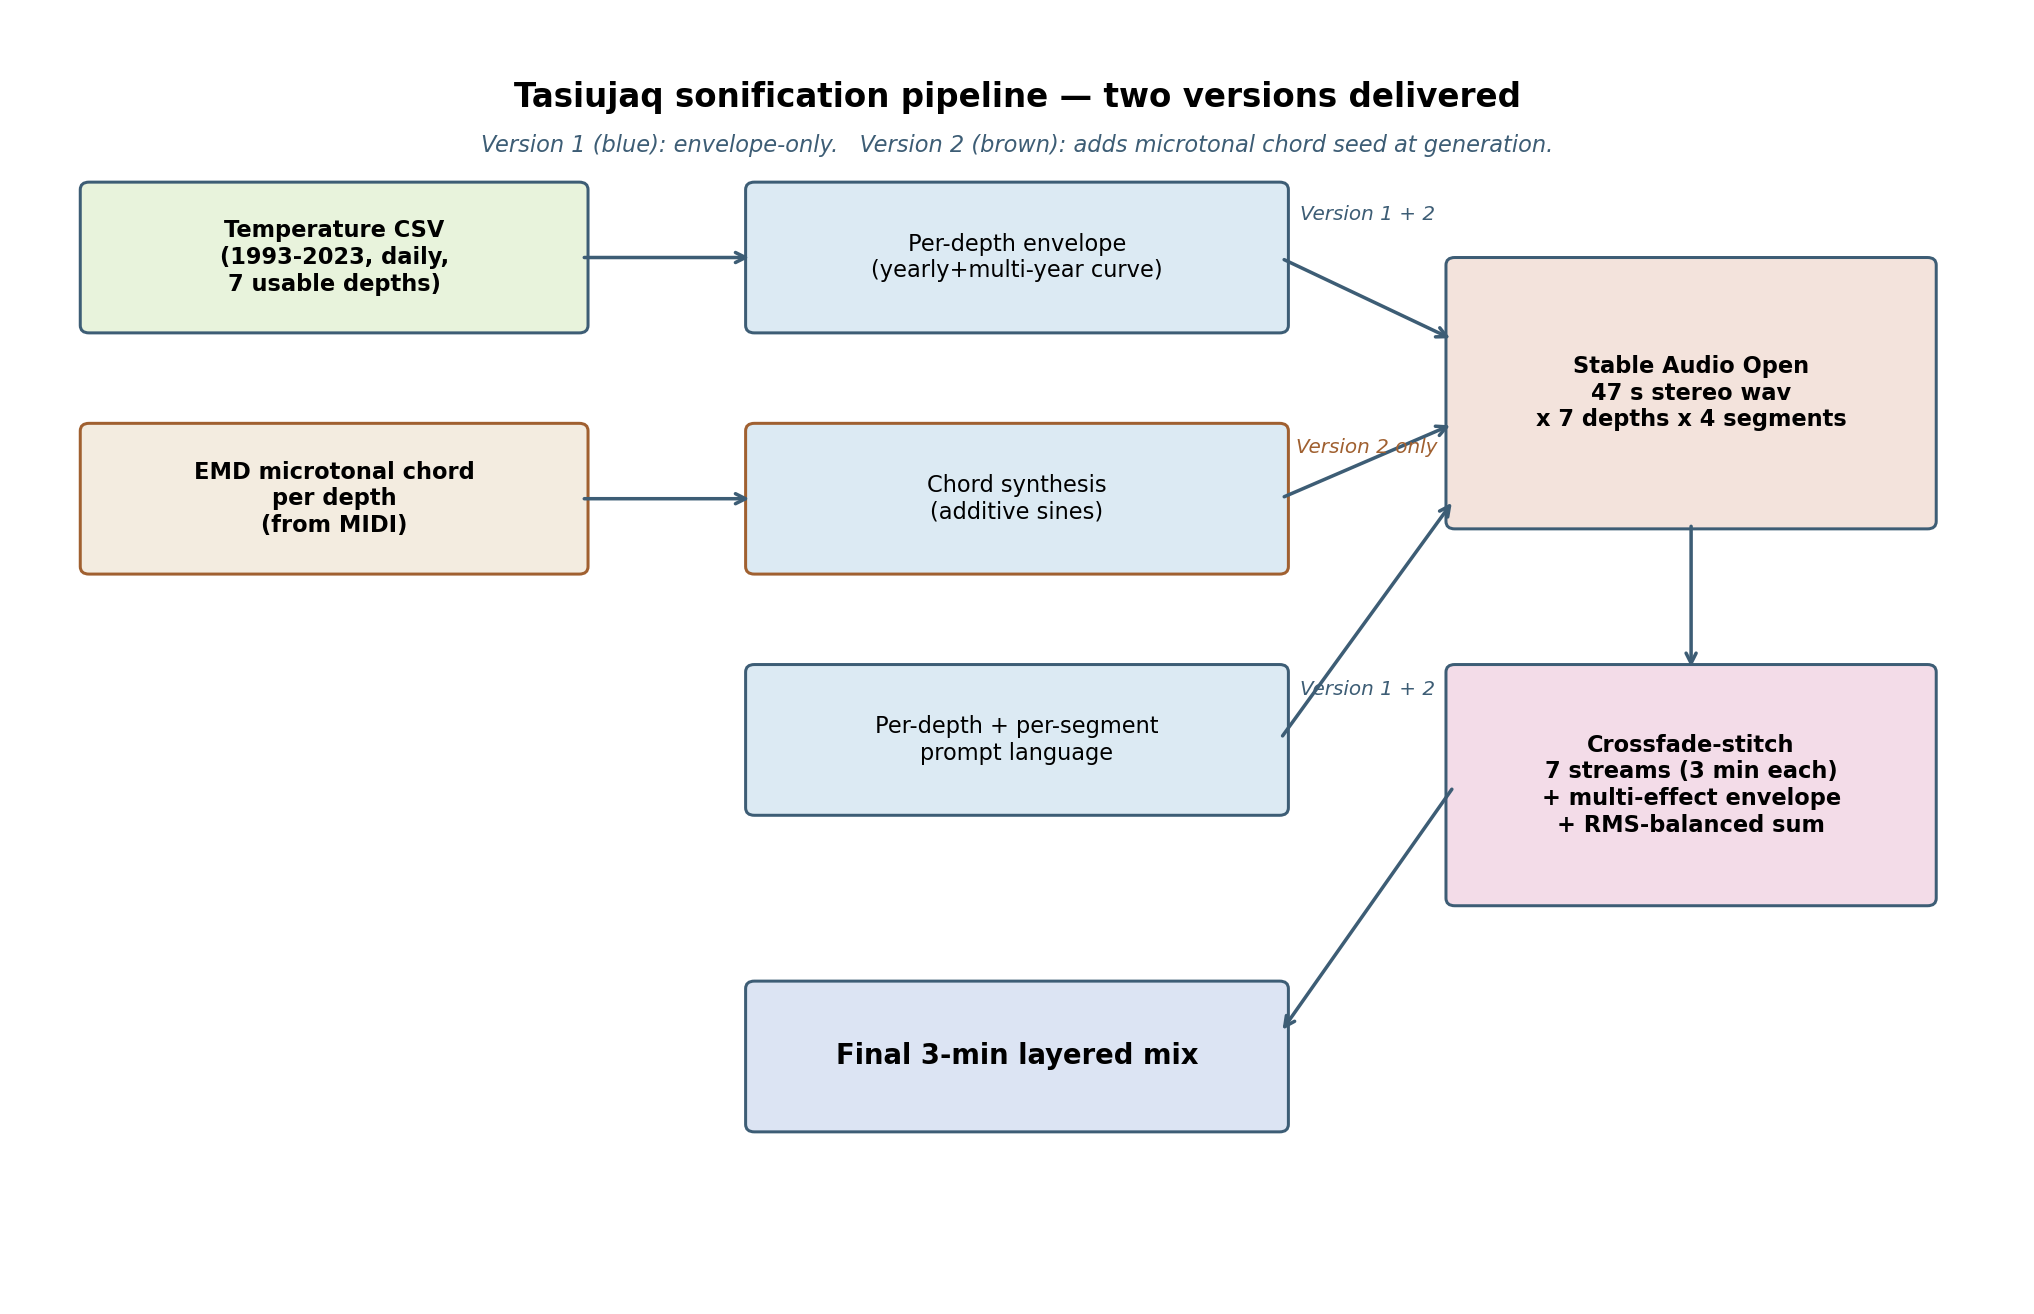
\includegraphics[width=0.96\linewidth]{01_pipeline.png}
\end{figure}

\vspace{1.0em}
\begin{tcolorbox}[tldr]
\noindent\textbf{Résumé.}\enspace
Nous transformons 27~années de données journalières de température du sol
de Tasiujaq (1993--2023) en deux pièces orchestrales complémentaires de
3~minutes. Les deux pièces partagent les mêmes sept voix musicales (une
par profondeur de sol entre 200~cm et 1100~cm), le même choix
d'instrumentation guidé par texte, et la même étape de mise en forme par
enveloppe. Elles diffèrent dans la \emph{manière dont les données se
couplent à l'audio généré}~:

\medskip
\noindent\textbf{Version~1, sonification modulée par enveloppe.}\enspace
Le signal du sol sculpte chaque voix par un effet audio dédié~:
intensité, brillance, largeur stéréo, trémolo ou coupure de basses. Chaque
voix exprime donc les données dans une dimension sensorielle différente.

\medskip
\noindent\textbf{Version~2, sonification ancrée par accord microtonal.}\enspace
En plus des effets d'enveloppe, le contenu harmonique microtonal de chaque
profondeur (extrait par décomposition modale empirique, EMD) est injecté
directement dans le processus de diffusion du modèle d'IA comme amorce. Les
hauteurs générées par le modèle sont alors biaisées vers l'accord réel de
la profondeur. Les données se couplent ainsi à la musique à la fois dans
le temps (enveloppe) et dans le spectre (accord).
\end{tcolorbox}

\vfill
\begin{flushleft}
  {\sffamily\footnotesize\color{footergray}
  Symphonie Arctique. Note méthodologique sur la création de la trame sonore IA.\\
  Édition à deux versions, préparée à partir des données et du code du projet.}
\end{flushleft}

\clearpage

% ---------- TABLE DES MATIÈRES ----------
\thispagestyle{cover}
\vspace*{1em}
\renewcommand{\contentsname}{Table des matières}
\tableofcontents
\vfill
\clearpage

\setcounter{page}{1}

% ============================================================================
\section{Les données source}
% ============================================================================

L'entrée est un fichier CSV de températures du sol mesurées à quatorze
profondeurs, entre $0$~cm (surface) et $1100$~cm (onze mètres sous terre),
à Tasiujaq, Nunavik. Les mesures sont journalières et couvrent
26{,}7~années (9{\,}748~jours, d'août~1993 à 2023). Sept des quatorze
profondeurs ont une couverture suffisamment continue pour être utilisables
dans la pièce~: $200$, $300$, $400$, $500$, $700$, $900$ et $1100$~cm.

Les profondeurs racontent des histoires physiques radicalement différentes.
Près de la surface, le sol suit les saisons de manière agressive : le
réchauffement estival pousse les températures au-dessus de
$+20\,^{\circ}\mathrm{C}$, tandis que l'air hivernal les fait chuter sous
$-30\,^{\circ}\mathrm{C}$. La chaleur diffuse lentement dans le sol, donc
chaque mètre supplémentaire de profondeur lisse et retarde ce signal.
À $11$~m de profondeur, les températures oscillent étroitement entre
$-5$ et $-4\,^{\circ}\mathrm{C}$ toute l'année. C'est le pergélisol,
presque immobile sur les 27~années de l'enregistrement.

Une entrée complémentaire est aussi disponible~: une décomposition modale
empirique (\emph{Empirical Mode Decomposition}, EMD) du même signal de
sol, exportée en fichier MIDI microtonal. Pour chaque profondeur utilisable,
l'analyse EMD produit 8 à 11~fréquences réparties sur environ huit octaves,
soit un << accord >> par profondeur qui caractérise sa structure harmonique
interne. La plus basse de ces fréquences se situe toujours autour de
28--32~Hz; cette fondamentale sub-grave commune reflète la tendance
pluridécennale de la température, à laquelle toutes les profondeurs
finissent par répondre.

\pullquote{Sol volatil $\to$ voix expressive. Sol stable $\to$ bourdon.}

% ============================================================================
\section{De la profondeur à la voix}
% ============================================================================

Chacune des sept profondeurs utilisables se voit attribuer sa propre voix
musicale : un instrument ou une couche vocale décrits en prose et fournis
au modèle d'IA comme prompt textuel. Les voix sont délibérément réparties
sur des bandes de fréquences et des rôles distincts, pour qu'elles se
superposent de manière transparente au lieu de se gêner dans une même
plage.

\begin{figure}[H]
  \centering
  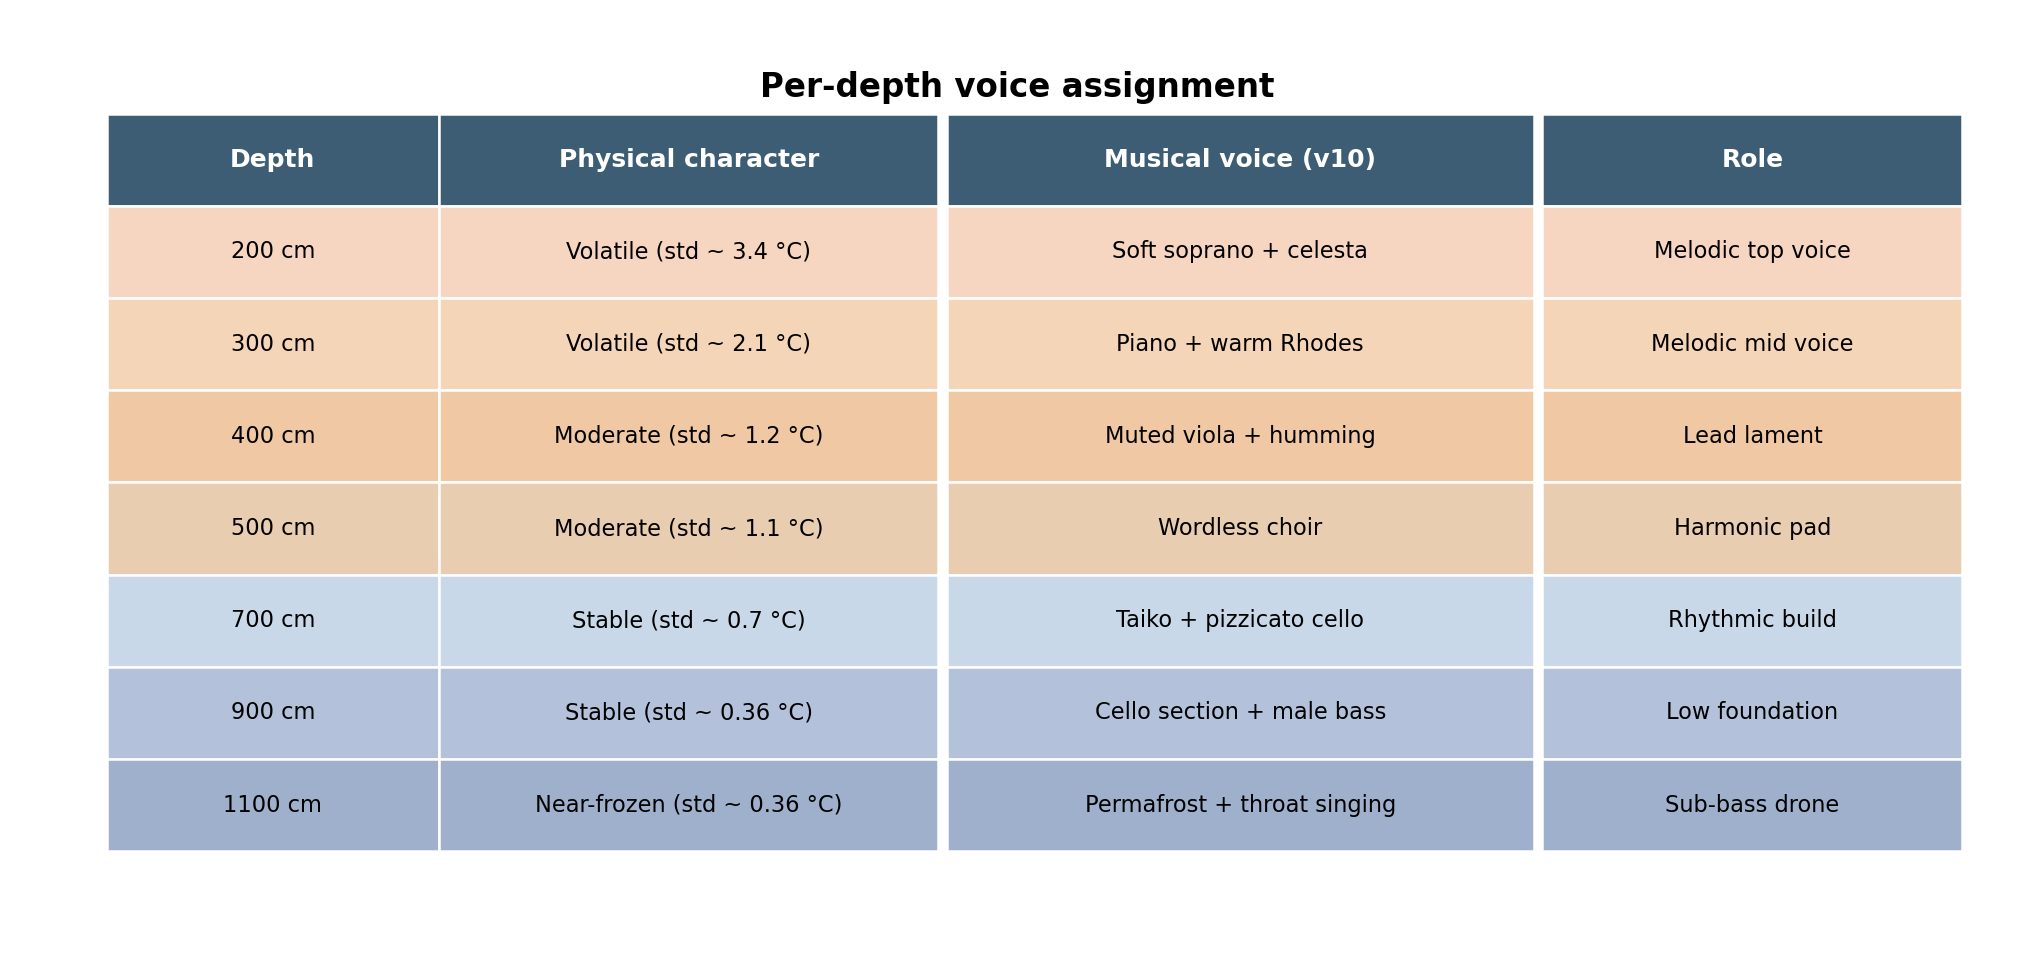
\includegraphics[width=\linewidth]{02_depth_voices.png}
  \caption{Attribution des voix par profondeur, partagée par les deux
  versions. Les tons chauds en haut sont les plus expressifs et
  mélodiques; les tons froids en bas tiennent le bourdon de fondation. Les
  pistes de surface contiennent les éléments les plus délicats et
  transitoires (voix, célesta); les pistes profondes sont soutenues et
  dans le registre grave.}
  \label{fig:depthvoices}
\end{figure}

% ============================================================================
\section{Cartographier 27 années sur 3 minutes}
% ============================================================================

La sortie maximale architecturale du modèle audio par IA est de 47~secondes.
Pour produire une pièce de 3~minutes, nous découpons l'audio en quatre
segments de 47~secondes superposés par fondu enchaîné (fondus à puissance
constante de 3~secondes, donnant $4 \times 47 - 3 \times 3 \approx 179$~s).
Nous tirons parti de cette contrainte~: chaque segment est alimenté par
une tranche différente d'environ 6{,}7~années du signal de sol, de sorte
que la tendance pluridécennale de réchauffement est inscrite dans la
progression musicale.

\begin{figure}[H]
  \centering
  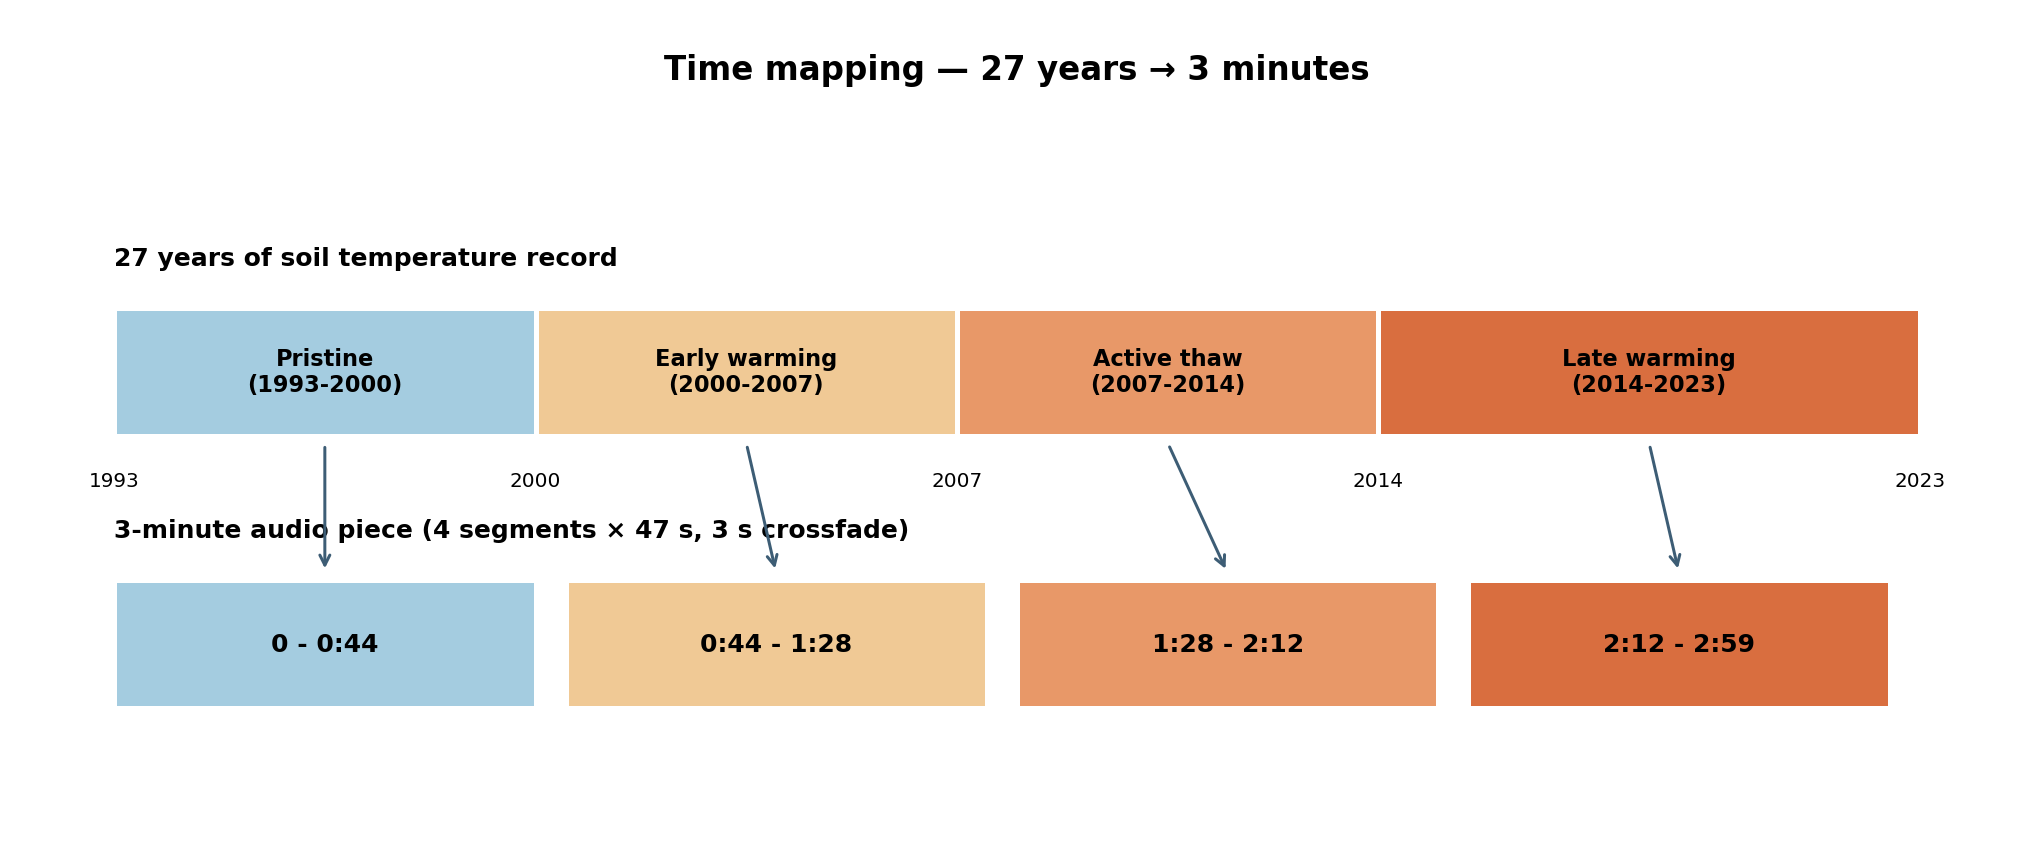
\includegraphics[width=\linewidth]{03_segments_timeline.png}
  \caption{Cartographie temporelle. Les 27~années d'enregistrement sont
  divisées en quatre fenêtres d'environ 6{,}7~années. Chaque fenêtre
  pilote un segment audio d'environ 47~s; les quatre segments sont ensuite
  reliés par fondu enchaîné dans la pièce finale d'environ 3~minutes. Les
  descripteurs de prompt évoluent en parallèle : << intact >> au début,
  << dégel actif >> au milieu, << réchauffement tardif >> à la fin.}
  \label{fig:timeline}
\end{figure}

\begin{tcolorbox}[note,title={\textbf{Chaque segment couvre ${\sim}6{,}7$ années, pas 1}}]
Parce que chaque segment de 47~secondes est piloté par environ
6{,}7~années de données journalières, chaque segment contient environ sept
cycles saisonniers du signal de sol. L'enveloppe oscille donc à la fois à
une échelle pluriannuelle lente (la tendance climatique) et à une échelle
annuelle plus rapide (les saisons) dans chaque fenêtre de 47~secondes.
\end{tcolorbox}

% ============================================================================
\section{Le mécanisme partagé~: l'extraction d'enveloppe}
\label{sec:envelope}
% ============================================================================

Les deux versions partagent la même première étape~: pour chaque
profondeur et chaque segment, la courbe réelle de température est
convertie en une \emph{enveloppe}, soit une courbe unique dans $[0, 1]$ qui
suit le signal du sol dans le temps. C'est cette enveloppe qui sculpte
l'audio généré par l'IA dans la deuxième étape.

\begin{figure}[H]
  \centering
  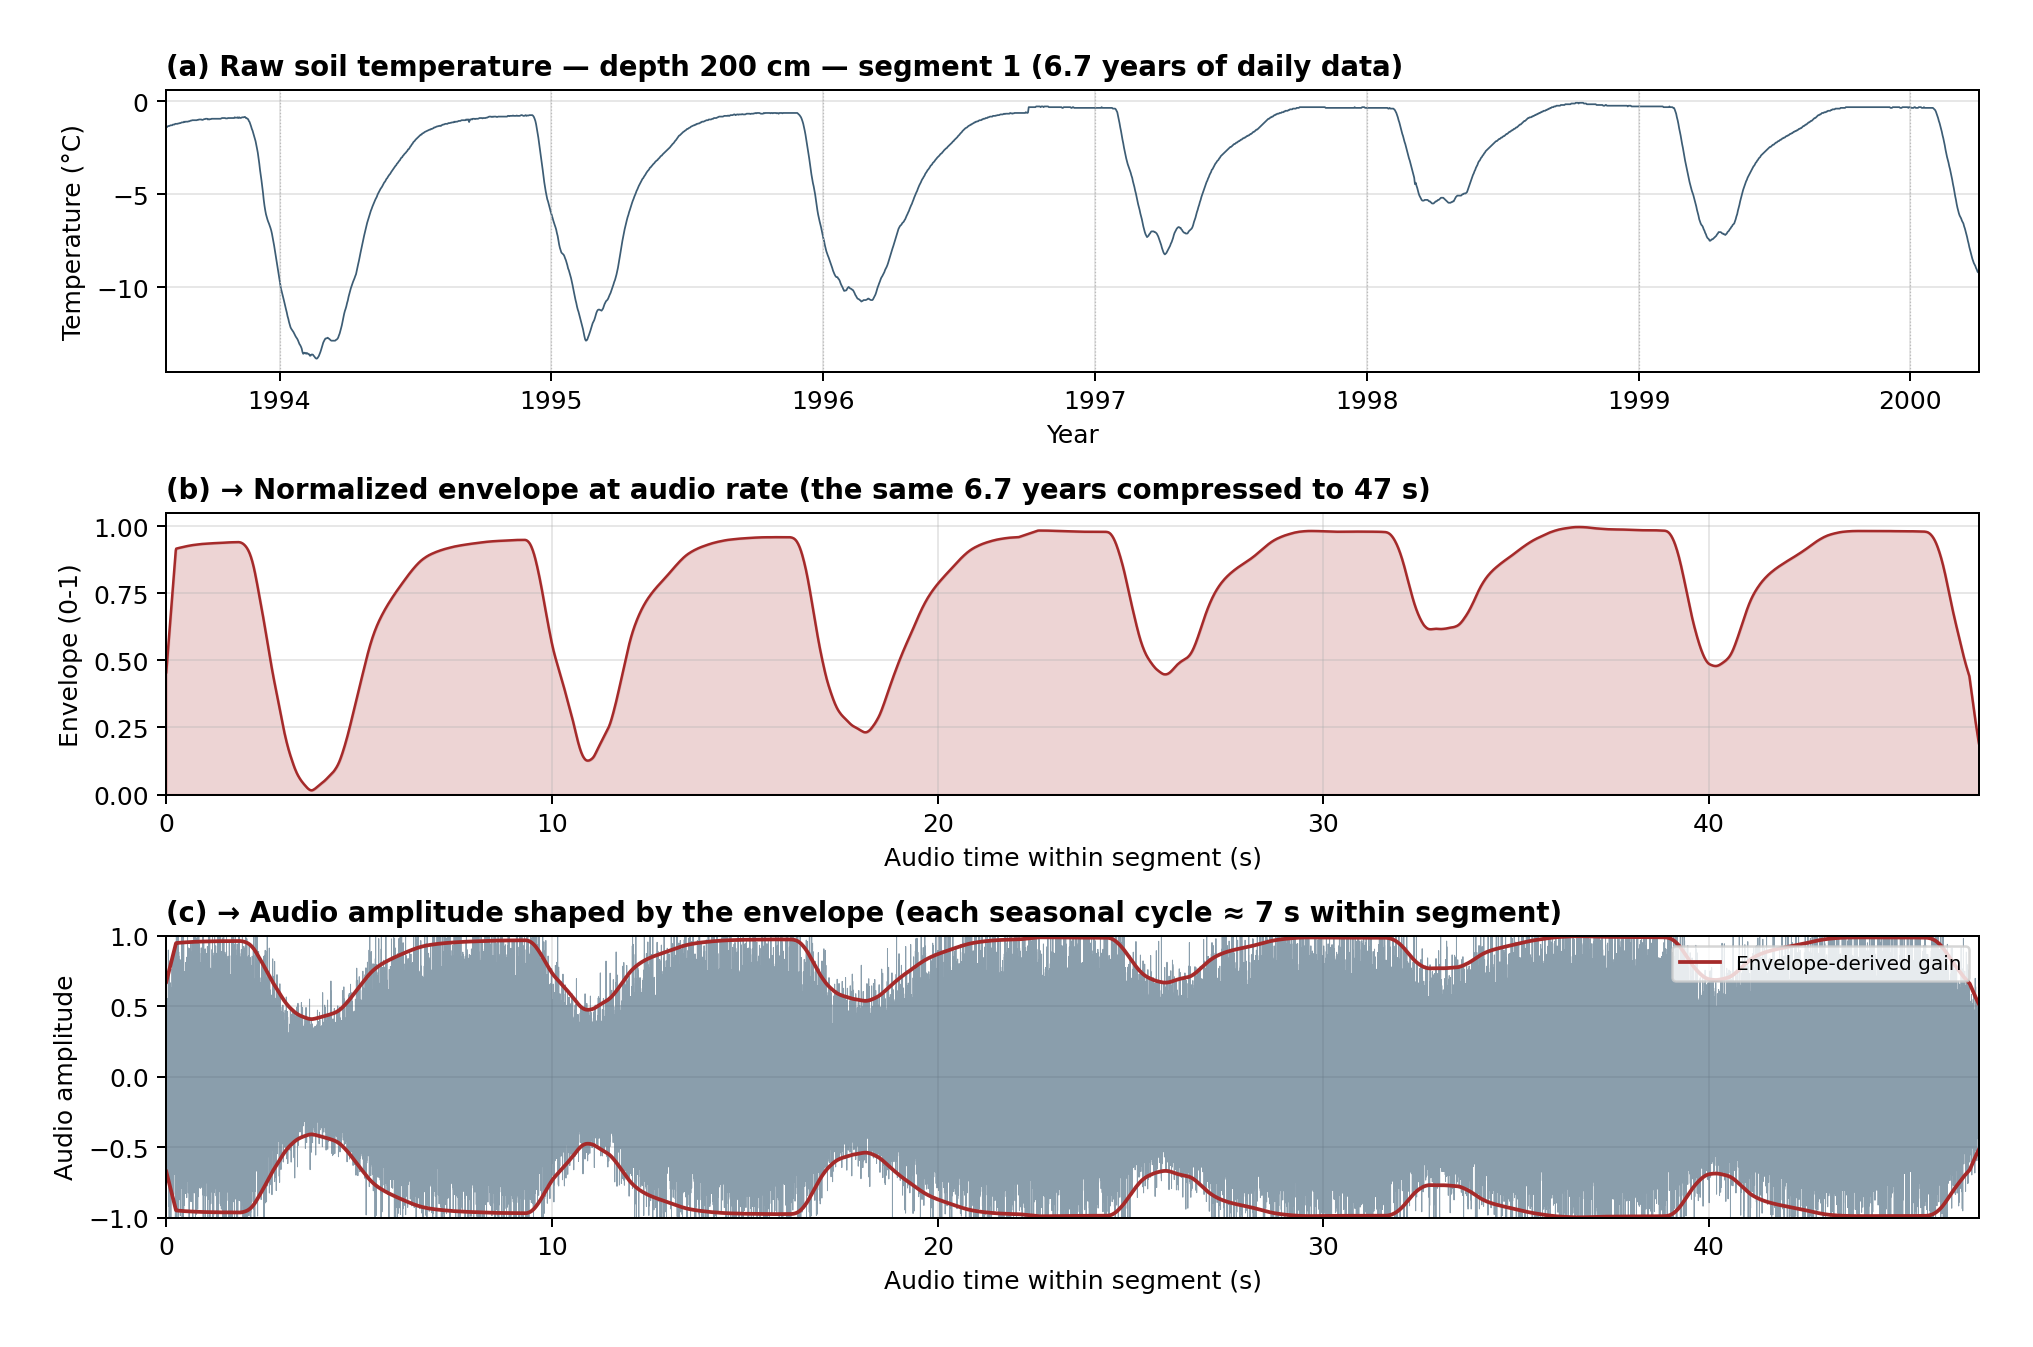
\includegraphics[width=\linewidth]{04_envelope_concept.png}
  \caption{La transformation en trois étapes, profondeur 200~cm, premier
  segment (1993--2000). \textbf{(a)}~Environ 6{,}7~années de données de
  température journalière. Sept cycles saisonniers sont clairement
  visibles. Les pointillés verticaux marquent le 1\ier{}~janvier; les
  creux tombent vers janvier (hiver), les pics au milieu d'année (été).
  \textbf{(b)}~La même forme est normalisée dans $[0,1]$, lissée, et
  rééchantillonnée sur la grille temporelle audio; chaque année occupe
  environ 7~secondes dans le segment de 47~secondes. \textbf{(c)}~L'enveloppe
  sculpte un signal audio synthétisé~: intensité et autres effets respirent
  au rythme des saisons.}
  \label{fig:envelope}
\end{figure}

L'audio que l'enveloppe vient mettre en forme est produit par \emph{Stable
Audio Open~1.0}, un modèle texte-vers-audio à poids ouverts exécuté
localement sur un seul GPU. Pour chaque couple profondeur~$\times$~segment,
nous écrivons un prompt sur mesure décrivant l'instrument de la voix, son
registre et son humeur propre au segment. Avec sept profondeurs et quatre
segments par profondeur, le modèle est invoqué 28~fois par pièce. La
génération est déterministe pour une graine aléatoire fixée.

\clearpage

% ============================================================================
\section{Version~1 : sonification modulée par enveloppe}
\label{sec:v1}
% ============================================================================

\begin{tcolorbox}[v1box]
\textbf{Version~1 en une ligne.}\enspace
L'IA génère chaque voix à partir d'un prompt textuel. L'enveloppe de
température de la profondeur pilote ensuite \emph{un} effet audio
signature sur cette voix, choisi pour que chaque voix exprime les
données dans une dimension sensorielle différente.
\end{tcolorbox}

\subsection{Acheminement des effets par profondeur}

L'enveloppe d'amplitude est toujours appliquée (l'intensité monte et
descend avec la chaleur). En plus, chaque profondeur reçoit un effet
supplémentaire adapté à sa voix. L'acheminement est intentionnel~: les
voix mélodiques et brillantes reçoivent un effet qui fait varier leur
brillance ou leur présence spatiale; les bourdons de fondation reçoivent
un effet sur les basses qui permet d'entendre la basse << dégeler >> à
mesure que le sol se réchauffe; les voix rythmiques gardent uniquement
l'amplitude, pour que l'auditeur sente encore clairement le rythme.

\begin{tabularx}{\linewidth}{@{}>{\sffamily}l L L@{}}
  \toprule
  \textbf{Profondeur} & \textbf{Voix} & \textbf{Effet piloté par l'enveloppe (froid $\to$ chaud)} \\
  \midrule
  200~cm  & Soprano + célesta                 & \textbf{Largeur stéréo.} Intime $\leftrightarrow$ large. \\
  300~cm  & Piano + Rhodes chaleureux         & \textbf{Coupure passe-bas.} Étouffée $\leftrightarrow$ brillante. \\
  400~cm  & Alto en sourdine + voix fredonnée & \textbf{Profondeur de trémolo.} Stable $\leftrightarrow$ vibrant. \\
  500~cm  & Chœur sans paroles                & \textbf{Largeur stéréo.} Étroite $\leftrightarrow$ large. \\
  700~cm  & Taiko + voix de basse masculine   & Aucun (amplitude seule, pour préserver la clarté rythmique). \\
  900~cm  & Violoncelles + voix de basse      & \textbf{Coupure passe-haut.} Graves coupés $\leftrightarrow$ pleins. \\
  1100~cm & Pergélisol + chant diphonique     & Aucun (amplitude seule, bourdon subtil). \\
  \bottomrule
\end{tabularx}

\subsection{Implémentation}

Tous les filtres pilotés par l'enveloppe sont implémentés comme un fondu
échantillon par échantillon entre une version pré-filtrée et le signal
original, ce qui évite les transitoires audibles qu'un filtrage IIR
par blocs produirait quand la fréquence de coupure varie rapidement. Le
trémolo est un LFO basse fréquence dont la \emph{profondeur} est modulée
par l'enveloppe (stable au froid, vibrant au chaud). La largeur stéréo
module le rapport mid/side.

\pullquote{La même courbe de température sculpte sept voix, chacune à sa façon.}

% ============================================================================
\section{Version~2 : sonification ancrée par accord microtonal}
\label{sec:v2}
% ============================================================================

\begin{tcolorbox}[v2box]
\textbf{Version~2 en une ligne.}\enspace
Mêmes effets d'enveloppe que la Version~1, plus~: l'accord microtonal
issu de l'EMD pour cette profondeur est fourni au modèle d'IA comme
\emph{amorce} du processus de diffusion. Les hauteurs générées par le
modèle sont biaisées vers cet accord. Les données se couplent ainsi à la
musique à la fois dans le temps \emph{et} dans le spectre.
\end{tcolorbox}

\subsection{L'accord d'amorçage}

Pour chaque profondeur, les partiels extraits du MIDI microtonal sont
synthétisés comme un signal stéréo de 47~secondes par sommation de
sinusoïdes. Les partiels au-dessus de 2~kHz sont écartés (ils injecteraient
un contenu aigu agressif) et les partiels restants sont pondérés pour que
les fréquences les plus basses dominent.

\begin{figure}[H]
  \centering
  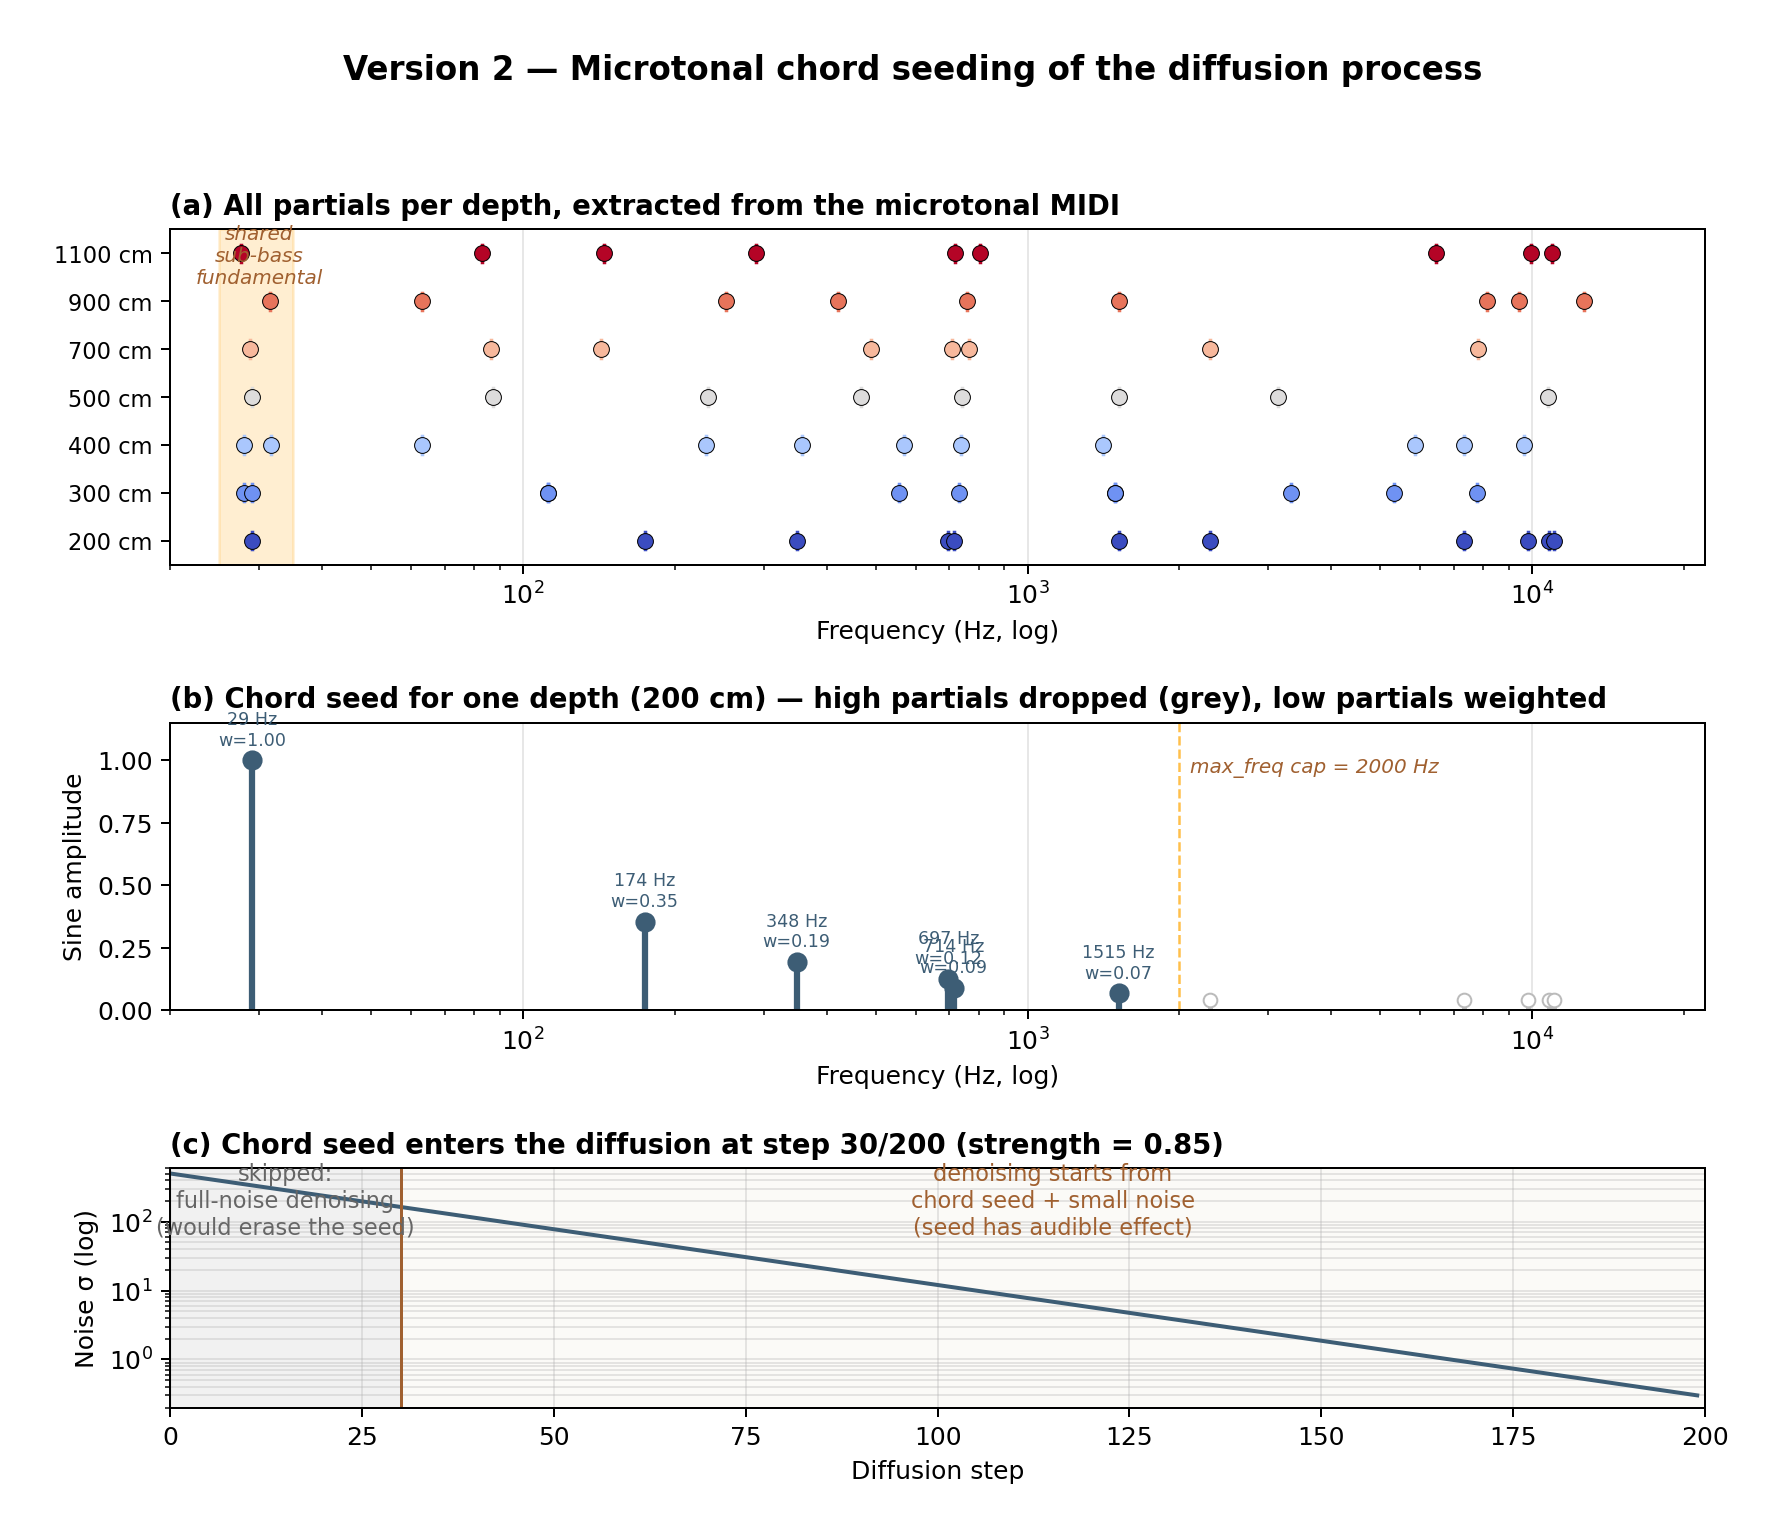
\includegraphics[width=\linewidth]{06_chord_seed.png}
  \caption{Construction et intégration de l'amorce d'accord pour la
  Version~2. \textbf{(a)}~Ensemble complet des partiels par profondeur,
  tels qu'extraits du MIDI microtonal. La bande orange marque la
  fondamentale sub-grave commune autour de $30$~Hz qui relie les sept
  profondeurs en une seule famille harmonique.
  \textbf{(b)}~Pour une profondeur (200~cm), les partiels conservés (en
  bleu) et écartés (en gris) après la coupure des aigus, avec les
  amplitudes utilisées dans la synthèse additive.
  \textbf{(c)}~Là où l'amorce entre dans le processus de diffusion~: au
  lieu de débruiter à partir de l'étape de bruit maximal (ce qui effacerait
  l'amorce), nous sautons les premiers 85~\% du calendrier de bruit et
  démarrons le débruitage à partir d'un bruit beaucoup plus faible. L'amorce
  a alors un effet audible sur le spectre final.}
  \label{fig:chordseed}
\end{figure}

\subsection{Comment l'amorce entre dans la diffusion}

Dans une génération texte-vers-audio standard, le modèle part d'un bruit
pur et débruite progressivement jusqu'à un audio qui correspond au prompt
textuel. Quand on fournit un audio initial, le pipeline standard ajoute
quand même un bruit de pleine amplitude par-dessus avant la première étape
de débruitage, ce qui efface presque toute influence de l'amorce. La
Version~2 utilise une variante de type \emph{img2img}~: le bruit ajouté à
l'amorce encodée est dimensionné à un niveau bien plus faible, et la
boucle de débruitage est raccourcie pour partir de ce point. Le modèle
opère désormais sur une représentation latente qui est réellement une
version bruitée de l'accord, et sa trajectoire de débruitage est attirée
vers le spectre de l'accord.

Un seul paramètre, la \emph{force} (\textit{strength}), contrôle le
compromis~: à $\textit{force}=1{,}0$ l'amorce est ignorée (comportement
standard); à des valeurs plus faibles, le modèle est de plus en plus
contraint au spectre de l'amorce. En pratique, nous utilisons
$\textit{force} \approx 0{,}85$, valeur à laquelle l'amorce façonne le
spectre sans écraser le contenu créatif du modèle.

\subsection{Ce qui est partagé avec la Version~1}

Le tableau d'acheminement multi-effet par profondeur de la
Section~\ref{sec:v1} est appliqué tel quel à l'audio de la Version~2.
L'amorce façonne \emph{les notes que joue le modèle}; les effets
d'enveloppe façonnent ensuite \emph{comment ces notes sont entendues dans
le temps}. Les données se couplent à la musique dans deux dimensions
orthogonales.

\clearpage

% ============================================================================
\section{Assemblage~: enchaînement et mixage}
% ============================================================================

Les quatre segments de chaque profondeur sont reliés par fondu enchaîné
(fondus à puissance constante de 3~secondes) en un flux unique d'environ
3~minutes. Les sept flux sont ensuite équilibrés en intensité et sommés
dans le mixage final. La même étape d'assemblage est utilisée pour les
deux versions.

\begin{figure}[H]
  \centering
  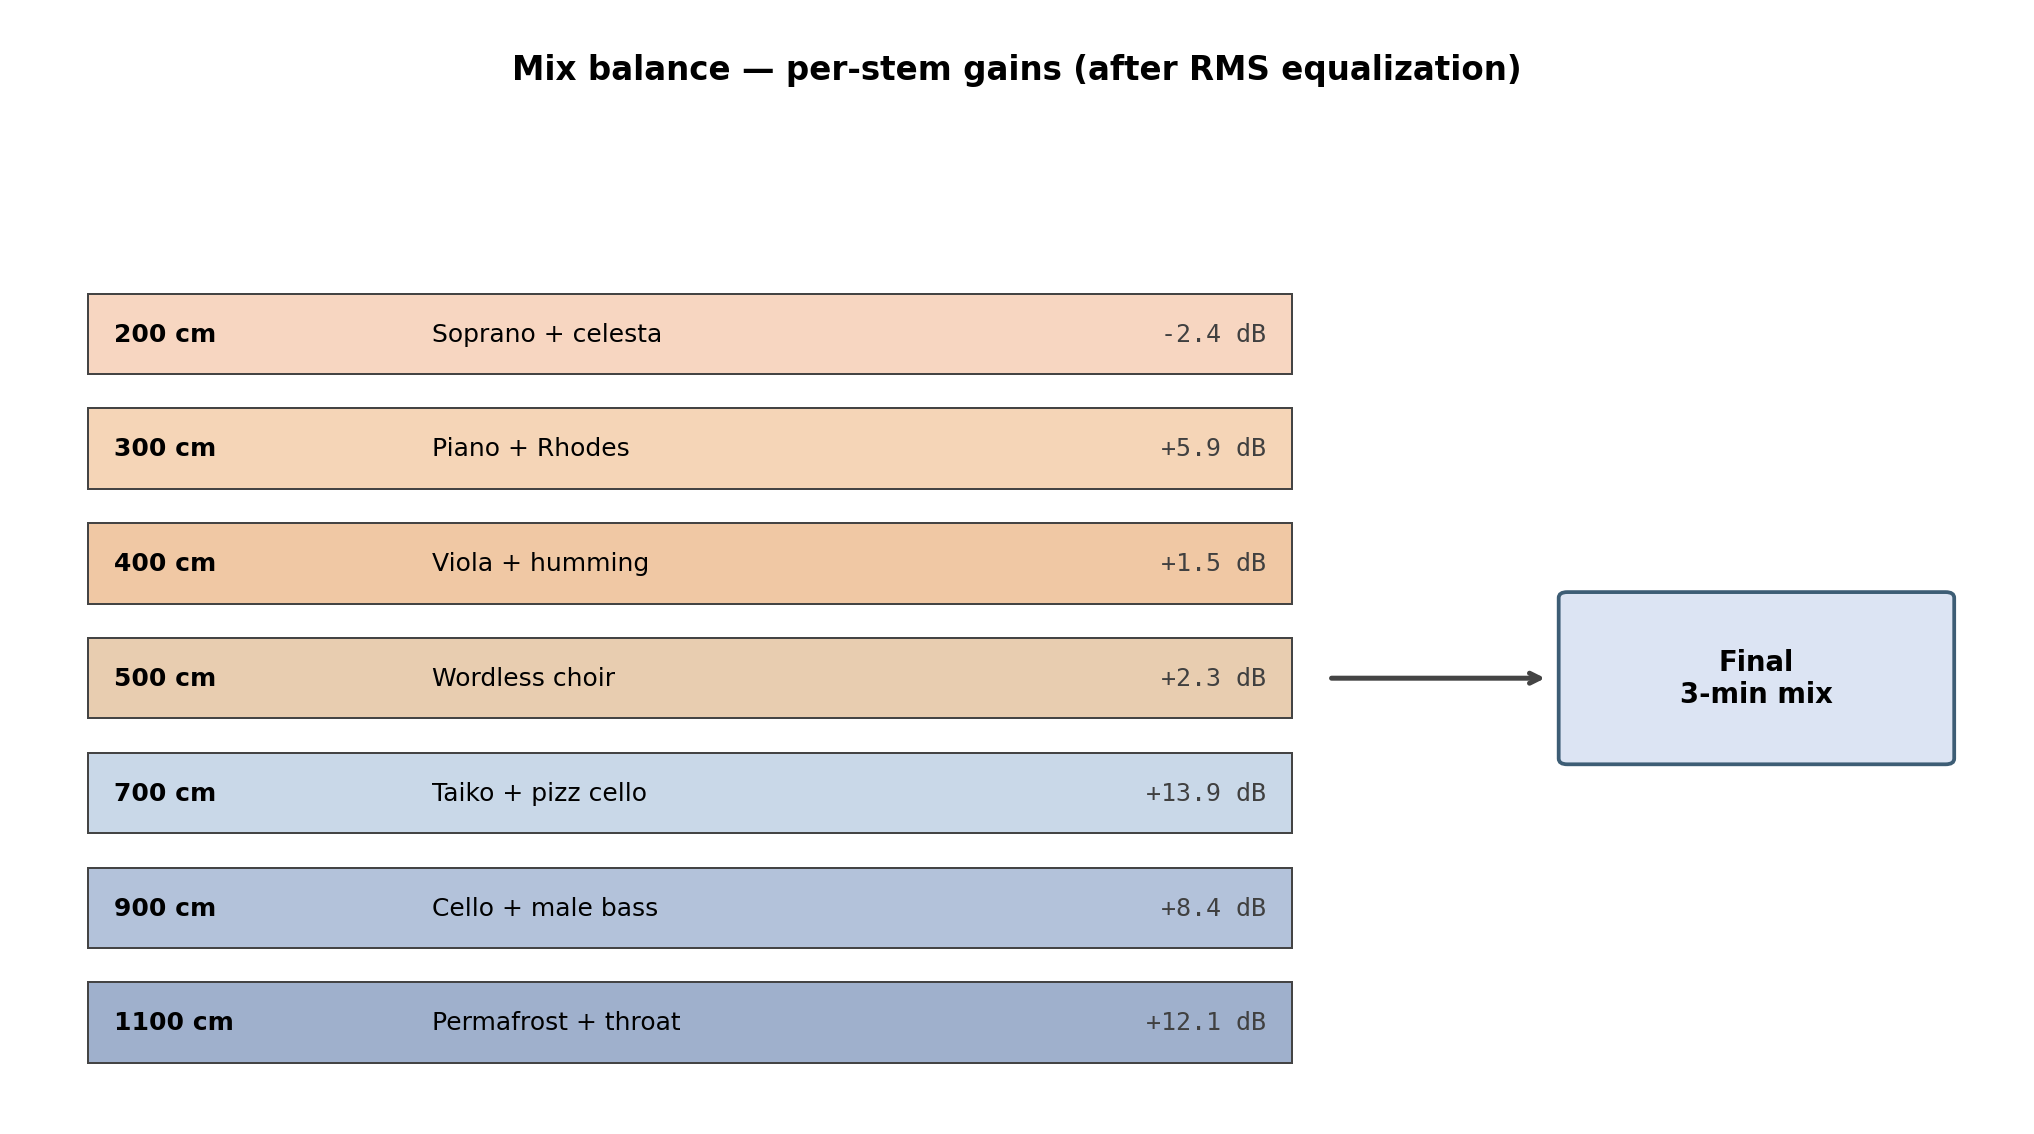
\includegraphics[width=\linewidth]{05_mix_stack.png}
  \caption{Équilibre du mixage. Les sept flux et leurs gains finaux dans
  les mixages livrés. Les pistes éparses ou transitoires (par exemple les
  taiko ou la sub-basse du pergélisol) reçoivent des amplifications plus
  fortes (jusqu'à $+12$~dB) pour rejoindre perceptivement les pistes denses
  et soutenues (comme le chœur). Les valeurs en dB à côté de chaque piste
  sont le gain total appliqué par un processus en deux étapes~:
  égalisation RMS (qui remonte les pistes éparses au niveau cible commun)
  et un petit ajustement manuel de fader par piste.}
  \label{fig:mix}
\end{figure}

% ============================================================================
\section{Feuille de route}
% ============================================================================

\subsubsection{Enveloppes multi-IMF}
Le signal de température de chaque profondeur peut lui-même être décomposé
par EMD en une courte liste de composantes fréquentielles (journalière,
saisonnière, pluriannuelle). Acheminer \emph{différents} IMFs vers des
effets différents sur une même voix (par exemple la tendance
pluriannuelle pilotant la coupure du filtre et le cycle saisonnier
pilotant l'intensité) donnerait trois flux de contrôle pilotés par les
données par profondeur au lieu d'un seul. Aucun calcul d'IA supplémentaire
nécessaire; seulement une itération de l'étape de mise en forme par
enveloppe.

\subsubsection{Voie~B : génération conditionnée par enveloppe}
Une extension plus ambitieuse consiste à faire en sorte que l'IA elle-même
planifie ses dynamiques pour que la courbe d'intensité naturelle de l'audio
généré corresponde déjà à l'enveloppe du sol, plutôt que d'appliquer
l'enveloppe après coup. C'est réalisable par optimisation au moment de
l'inférence du bruit latent initial (méthodes de type DITTO). Le coût en
calcul est environ $10\times$ le pipeline actuel.

\subsubsection{Voie~B$^{\!+}$ : conditionnement multi-cible}
La même optimisation à l'inférence peut viser à la fois l'enveloppe
\emph{et} le spectre simultanément, en utilisant l'amorce d'accord comme
cible spectrale et la courbe de température comme cible d'enveloppe. Cela
unifierait les Versions~1 et~2 en une seule passe de conditionnement
plutôt qu'un pipeline en deux étapes.

\vspace{2em}
\begin{flushleft}
{\sffamily\small\color{footergray}%
\textbf{Provenance.}\enspace%
Données source~: surveillance du pergélisol à Tasiujaq (1993--2023).
Modèle audio~: Stable Audio Open~1.0 (Stability~AI).
Implémentation du pipeline~: ce projet, Python~3.12 avec
\texttt{diffusers}, \texttt{scipy}, \texttt{matplotlib}.
Mise en page \LaTeX{} (Tectonic), Linux Libertine.\par
\medskip
\textbf{Fichiers livrés.}\enspace
Version~1~: \texttt{outputs/mix\_3min\_v10\_3\_balanced.wav}.\\
Version~2~: \texttt{outputs/mix\_3min\_v15\_2\_balanced.wav}.}
\end{flushleft}

\end{document}
